\documentclass[aspectratio=169,11pt]{beamer}
\usepackage[utf8]{inputenc}
\usepackage[T1]{fontenc}
\usepackage[scaled=1.02]{helvet}
\renewcommand{\familydefault}{\sfdefault}
\usepackage{tikz}
\usepackage{array}
\usetikzlibrary{arrows.meta,positioning,calc,fit,shapes.misc}

% ---- the game palette ----
\definecolor{gmbg}{HTML}{0B0710}     % background
\definecolor{gmpanel}{HTML}{1C1119}  % panel
\definecolor{coral}{HTML}{E08D6D}    % accent coral
\definecolor{cream}{HTML}{F2E8DC}    % text cream
\definecolor{gold}{HTML}{FFD87A}     % gold
\definecolor{teal}{HTML}{7FE9D6}     % teal

\setbeamercolor{background canvas}{bg=gmbg}
\setbeamercolor{normal text}{fg=cream}
\setbeamercolor{structure}{fg=coral}
\setbeamercolor{frametitle}{fg=cream,bg=gmbg}
\setbeamercolor{title}{fg=cream}
\setbeamercolor{itemize/enumerate body}{fg=cream}
\setbeamercolor{itemize/enumerate subbody}{fg=cream}
\setbeamerfont{frametitle}{size=\LARGE,series=\bfseries}
\setbeamerfont{title}{size=\Huge,series=\bfseries}
\setbeamertemplate{navigation symbols}{}
\setbeamertemplate{itemize item}{\textcolor{coral}{\rule[0.42ex]{0.72ex}{0.72ex}}}
\setbeamertemplate{itemize subitem}{\textcolor{gold}{--}}
\setbeamertemplate{frametitle}{%
  \vspace*{0.8em}\usebeamerfont{frametitle}\insertframetitle\par
  \vspace{0.28em}{\color{coral}\hrule height 1.4pt}\vspace{0.35em}}
\setbeamertemplate{footline}{\hfill{\color{cream!45!gmbg}\scriptsize\insertframenumber\hspace{2em}}\vspace{0.6em}}
\setbeamersize{text margin left=1.0cm,text margin right=1.0cm}

\newcommand{\kicker}[1]{{\color{coral}\scriptsize\bfseries\MakeUppercase{#1}}\\[0.3em]}
\newcommand{\dimt}[1]{{\color{cream!62!gmbg}#1}}
\newcommand{\goldb}[1]{{\color{gold}\textbf{#1}}}
\newcommand{\tealb}[1]{{\color{teal}\textbf{#1}}}
\newcommand{\lbl}[1]{{\scriptsize\color{cream!62!gmbg}\MakeUppercase{#1}}}
\newcommand{\stepno}[1]{{\color{gold}\bfseries #1}\,}
\newcommand{\says}[1]{\textcolor{coral}{\emph{``#1''}}}

% shared tikz styles
\tikzset{
  panelbox/.style={draw=cream!22!gmbg, fill=gmpanel, rounded corners=3pt,
                   inner sep=7pt, align=center, text=cream, font=\small},
  gembox/.style={draw=coral, line width=1.3pt, fill=gmpanel, rounded corners=3pt,
                 inner sep=7pt, align=center, text=cream, font=\small},
  codebox/.style={draw=teal, line width=1.3pt, fill=gmpanel, rounded corners=3pt,
                  inner sep=7pt, align=center, text=cream, font=\small},
  goldbox/.style={draw=gold, line width=1.3pt, fill=gmpanel, rounded corners=3pt,
                  inner sep=7pt, align=center, text=cream, font=\small},
  arr/.style={-{Stealth[length=2.8mm]}, line width=1.2pt, color=coral},
  tarr/.style={-{Stealth[length=2.8mm]}, line width=1.2pt, color=teal},
  garr/.style={-{Stealth[length=2.8mm]}, line width=1.2pt, color=gold}}

\title{Prometheus Citadel}
\author{}
\date{}

\begin{document}

% ================================================================ 1 · TITLE
\begin{frame}
  \begin{center}
    \vspace{1.1em}
    \kicker{Kaggle · Build with AI --- Gemma Hackathon · GDG Windsor}
    {\fontsize{40}{44}\selectfont\bfseries\color{cream} GEMMA \textcolor{coral}{MONSTERS}\par}
    \vspace{0.55em}
    {\Large A monster-battling citadel with a real tutoring agent inside.\par}
    \vspace{0.55em}
    {\color{gold}\large Five monsters are out to get the student --- each with its own
     favourite way of tripping them into a mistake.\par}
    \vspace{0.35em}
    \dimt{Grade 9 EQAO mathematics. Gemma through Ollama, entirely on one laptop.}\par
    \vspace{1.4em}
    {\small Gokulakrishnan \,\textcolor{coral}{·}\, Padmanabha \,\textcolor{coral}{·}\, Taha \,\textcolor{coral}{·}\, Naimah \,\textcolor{coral}{·}\, Amarah}
  \end{center}
\end{frame}

% ================================================================ 2 · PROBLEM
\begin{frame}{A wrong answer is not noise. It is a sentence.}
  \begin{center}
    \vspace{-0.15em}
    {\fontsize{26}{30}\selectfont
      $\dfrac{2}{3}+\dfrac{1}{4}\;=\;$\textcolor{coral}{$\dfrac{3}{7}$}\par}
    \vspace{0.25em}
    {Tops with tops, bottoms with bottoms. Feels tidy. Completely wrong.\par}
    \vspace{0.35em}
    \resizebox{0.99\textwidth}{!}{%
    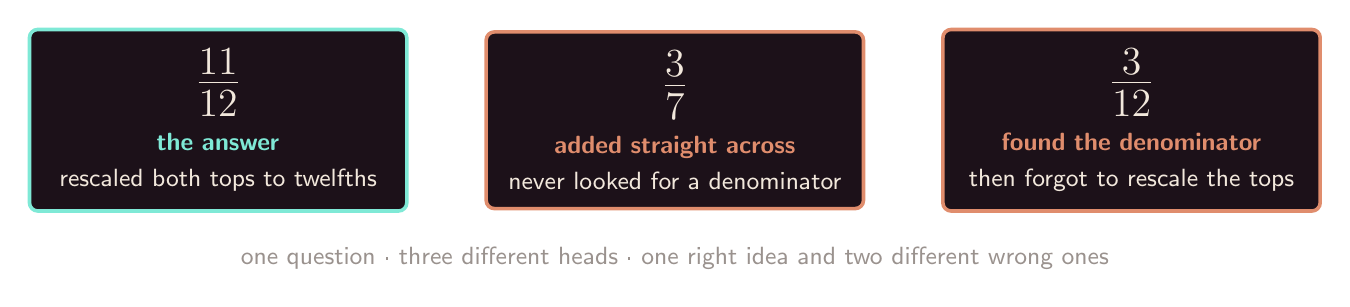
\begin{tikzpicture}[card/.style={text width=4.3cm, minimum height=2.1cm}]
      \node[codebox, card] (a) at (0,0)
        {{\fontsize{22}{24}\selectfont$\frac{11}{12}$}\\[5pt]
         \tealb{the answer}\\[2pt]
         \small rescaled both tops to twelfths};
      \node[gembox, card] (b) at (5.8,0)
        {{\fontsize{22}{24}\selectfont$\frac{3}{7}$}\\[5pt]
         \textcolor{coral}{\textbf{added straight across}}\\[2pt]
         \small never looked for a denominator};
      \node[gembox, card] (c) at (11.6,0)
        {{\fontsize{22}{24}\selectfont$\frac{3}{12}$}\\[5pt]
         \textcolor{coral}{\textbf{found the denominator}}\\[2pt]
         \small then forgot to rescale the tops};
      \node[font=\small, text=cream!62!gmbg] at (5.8,-1.75)
        {one question · three different heads · one right idea and two different wrong ones};
    \end{tikzpicture}}
    \vspace{0.45em}

    {\color{gold}\Large\bfseries A wrong answer is a specific wrong idea that feels right.\par}
    \vspace{0.25em}
    {\small\dimt{These two students do not need the same worksheet. They need different ideas found and beaten.}}
  \end{center}
\end{frame}

% ================================================================ 3 · MONSTERS
\begin{frame}{Five monsters, five favourite ways to trip you}
  \vspace{-0.15em}
  Each monster is out to get the student, and each has its own preferred trap.
  Below, in the student's own words, is what it wants them to believe.\par
  \vspace{0.4em}
  \begin{center}
  \resizebox{0.995\textwidth}{!}{%
  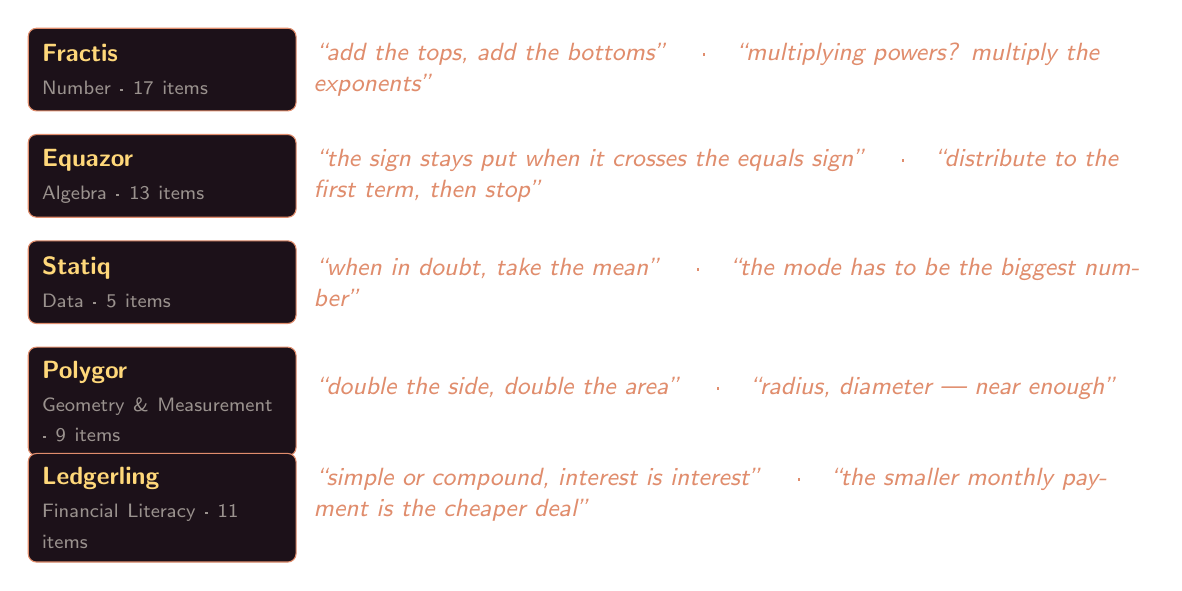
\begin{tikzpicture}[
     chip/.style={draw=coral, fill=gmpanel, rounded corners=3pt, inner sep=5pt,
                  text width=3.05cm, align=left, text=cream, font=\small,
                  minimum height=1.05cm},
     say/.style={align=left, text width=10.5cm, text=cream, font=\small,
                 inner sep=5pt, minimum height=1.05cm},
     every node/.append style={anchor=north west}]
    \node[chip] (c1) at (0,0)
      {\textbf{\color{gold}Fractis}\\[1pt]\scriptsize\color{cream!62!gmbg} Number · 17 items};
    \node[say] at (3.45,0)
      {\says{add the tops, add the bottoms} \quad\textcolor{coral}{·}\quad
       \says{multiplying powers? multiply the exponents}};
    \node[chip] (c2) at (0,-1.35)
      {\textbf{\color{gold}Equazor}\\[1pt]\scriptsize\color{cream!62!gmbg} Algebra · 13 items};
    \node[say] at (3.45,-1.35)
      {\says{the sign stays put when it crosses the equals sign} \quad\textcolor{coral}{·}\quad
       \says{distribute to the first term, then stop}};
    \node[chip] (c3) at (0,-2.70)
      {\textbf{\color{gold}Statiq}\\[1pt]\scriptsize\color{cream!62!gmbg} Data · 5 items};
    \node[say] at (3.45,-2.70)
      {\says{when in doubt, take the mean} \quad\textcolor{coral}{·}\quad
       \says{the mode has to be the biggest number}};
    \node[chip] (c4) at (0,-4.05)
      {\textbf{\color{gold}Polygor}\\[1pt]\scriptsize\color{cream!62!gmbg} Geometry \& Measurement · 9 items};
    \node[say] at (3.45,-4.05)
      {\says{double the side, double the area} \quad\textcolor{coral}{·}\quad
       \says{radius, diameter --- near enough}};
    \node[chip] (c5) at (0,-5.40)
      {\textbf{\color{gold}Ledgerling}\\[1pt]\scriptsize\color{cream!62!gmbg} Financial Literacy · 11 items};
    \node[say] at (3.45,-5.40)
      {\says{simple or compound, interest is interest} \quad\textcolor{coral}{·}\quad
       \says{the smaller monthly payment is the cheaper deal}};
  \end{tikzpicture}}
  \end{center}
  \vspace{0.35em}
  {\footnotesize Every line above is a \tealb{tag on a wrong option} in the bank. Pick that
   option and plain code reads the tag --- no model call --- and the trap is named on screen.\par}
\end{frame}

% ================================================================ 4 · JOURNEY
\begin{frame}{One session, start to finish}
  \begin{center}
  \resizebox{0.93\textwidth}{!}{%
  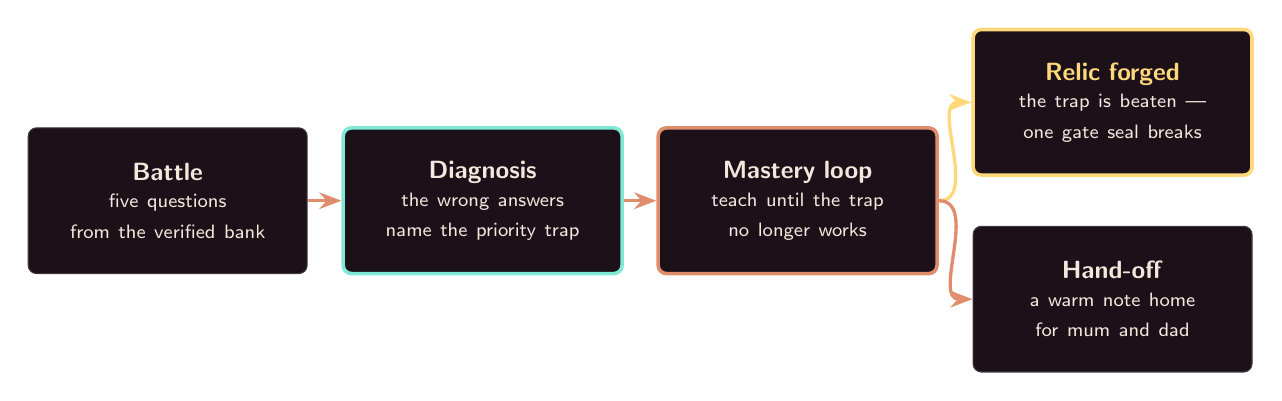
\begin{tikzpicture}[bx/.style={minimum height=1.85cm, text width=3.05cm, align=center}]
    \node[panelbox, bx] (fight) at (0,0)
      {\textbf{Battle}\\[2pt]\scriptsize five questions\\ \scriptsize from the verified bank};
    \node[codebox, bx] (diag) at (4.0,0)
      {\textbf{Diagnosis}\\[2pt]\scriptsize the wrong answers\\ \scriptsize name the priority trap};
    \node[gembox, bx] (loop) at (8.0,0)
      {\textbf{Mastery loop}\\[2pt]\scriptsize teach until the trap\\ \scriptsize no longer works};
    \node[goldbox, bx] (relic) at (12.0,1.25)
      {\textbf{\textcolor{gold}{Relic forged}}\\[2pt]\scriptsize the trap is beaten ---\\ \scriptsize one gate seal breaks};
    \node[panelbox, bx] (coll) at (12.0,-1.25)
      {\textbf{Hand-off}\\[2pt]\scriptsize a warm note home\\ \scriptsize for mum and dad};
    \draw[arr] (fight) -- (diag);
    \draw[arr] (diag) -- (loop);
    \draw[garr] (loop.east) to[out=0,in=180] (relic.west);
    \draw[arr] (loop.east) to[out=0,in=180] (coll.west);
  \end{tikzpicture}}
  \end{center}
  \vspace{0.7em}
  \begin{itemize}\setlength\itemsep{0.45em}
    \item The monster meets the student \textbf{by name}, and it \goldb{remembers}: Gemma writes
          its greeting from the real battle history on disk.
    \item Between battles: \textbf{ninety-second mental-maths skirmishes} against the Collector's
          three lieutenants.
    \item Beat all five monsters \,$\rightarrow$\, the golden gate opens \,$\rightarrow$\, \goldb{the rescue finale}.
  \end{itemize}
\end{frame}

% ================================================================ 5 · THE BANK
\begin{frame}{The bank is the ground truth}
  \large Ontario \goldb{MTH1W} --- the course behind the Grade 9 EQAO assessment.
  \textbf{55 items}, audited against the published expectations and the EQAO framework.\par
  \normalsize
  \vspace{0.45em}
  \begin{center}
  \resizebox{0.97\textwidth}{!}{%
  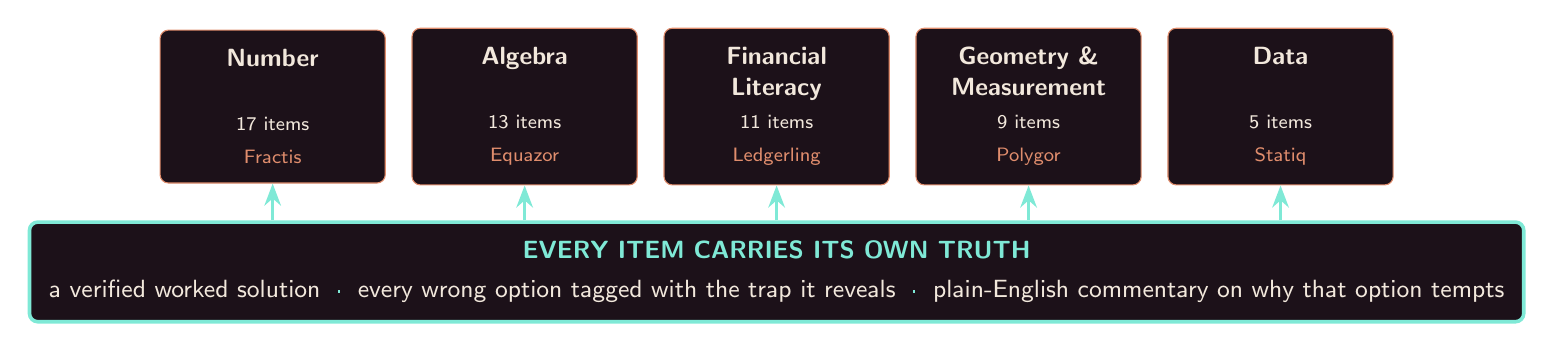
\begin{tikzpicture}[strand/.style={panelbox, draw=coral, minimum width=2.86cm,
                                     minimum height=1.75cm, font=\small}]
    \node[strand] (s1) at (0,0)
      {\textbf{Number}\\ \textbf{\phantom{Measurement}}\\[1pt]\scriptsize 17 items\\[1pt]\scriptsize\color{coral} Fractis};
    \node[strand] (s2) at (3.2,0)
      {\textbf{Algebra}\\ \textbf{\phantom{Measurement}}\\[1pt]\scriptsize 13 items\\[1pt]\scriptsize\color{coral} Equazor};
    \node[strand] (s3) at (6.4,0)
      {\textbf{Financial}\\ \textbf{Literacy}\\[1pt]\scriptsize 11 items\\[1pt]\scriptsize\color{coral} Ledgerling};
    \node[strand] (s4) at (9.6,0)
      {\textbf{Geometry \&}\\ \textbf{Measurement}\\[1pt]\scriptsize 9 items\\[1pt]\scriptsize\color{coral} Polygor};
    \node[strand] (s5) at (12.8,0)
      {\textbf{Data}\\ \textbf{\phantom{Measurement}}\\[1pt]\scriptsize 5 items\\[1pt]\scriptsize\color{coral} Statiq};
    \node[codebox, minimum width=15.7cm, font=\small] (bank) at (6.4,-2.1)
      {\tealb{EVERY ITEM CARRIES ITS OWN TRUTH}\\[3pt]
       a verified worked solution \;\textcolor{teal}{·}\;
       every wrong option tagged with the trap it reveals \;\textcolor{teal}{·}\;
       plain-English commentary on why that option tempts};
    \draw[tarr] (bank.north -| s1) -- (s1.south);
    \draw[tarr] (bank.north -| s2) -- (s2.south);
    \draw[tarr] (bank.north -| s3) -- (s3.south);
    \draw[tarr] (bank.north -| s4) -- (s4.south);
    \draw[tarr] (bank.north -| s5) -- (s5.south);
  \end{tikzpicture}}
  \end{center}
  \vspace{0.5em}
  {\footnotesize
   \goldb{The answer key is balanced 14 / 14 / 14 / 13 across A--D}, which removes the
   single-letter guessing edge --- always picking C scores no better than chance. The
   wrong-answer commentary is keyed to the \tealb{answer text}, never the option letter, so
   it stays true however the options are ordered. Retrieval is a table lookup, not a search:
   the payload wanted is an exact answer key.\par}
\end{frame}

% ================================================================ 6 · WORKED EXAMPLE, PART 1
\begin{frame}{One student, one trap: the battle question}
  \begin{center}
  \resizebox{0.93\textwidth}{!}{%
  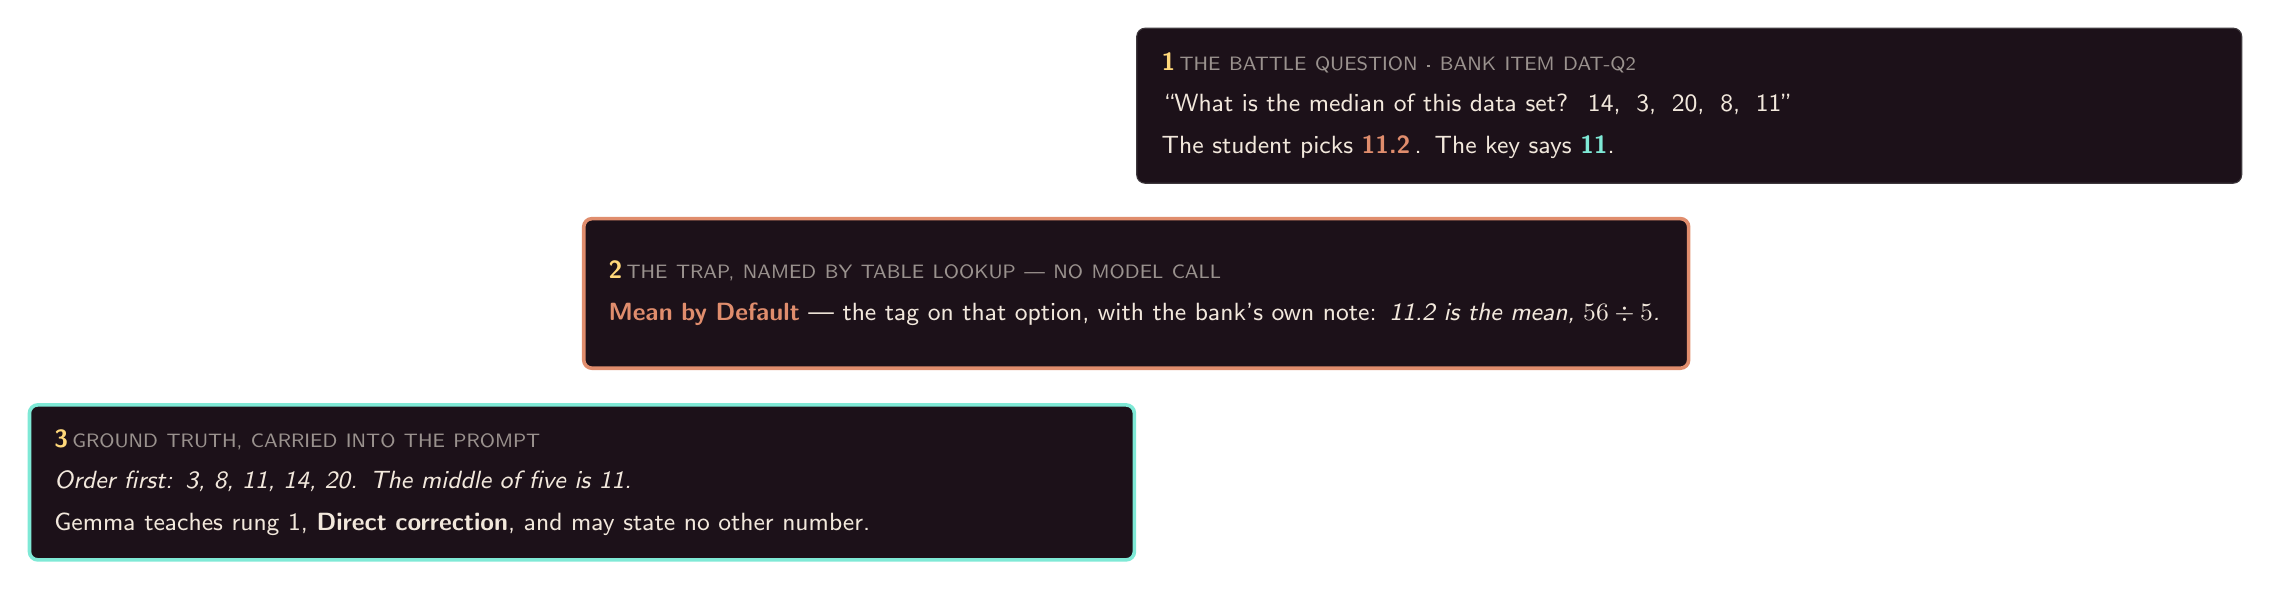
\begin{tikzpicture}[bx/.style={inner sep=9pt, align=left, font=\small,
                                 text width=13.4cm, minimum height=1.9cm},
                      every node/.append style={anchor=north west}]
    \node[panelbox, bx] (q) at (0, 0)
      {\stepno{1}\lbl{the battle question · bank item DAT-Q2}\\[4pt]
       ``What is the median of this data set? \;14, \;3, \;20, \;8, \;11''\\[4pt]
       The student picks \textcolor{coral}{\textbf{11.2}}\,. The key says \tealb{11}.};
    \node[gembox, bx, below=0.42cm of q.south west] (t)
      {\stepno{2}\lbl{the trap, named by table lookup --- no model call}\\[4pt]
       \textcolor{coral}{\textbf{Mean by Default}} --- the tag on that option, with the bank's
       own note: \emph{11.2 is the mean, $56 \div 5$.}};
    \node[codebox, bx, below=0.42cm of t.south west] (g)
      {\stepno{3}\lbl{ground truth, carried into the prompt}\\[4pt]
       \emph{Order first: 3, 8, 11, 14, 20. The middle of five is 11.}\\[4pt]
       Gemma teaches rung 1, \textbf{Direct correction}, and may state no other number.};
  \end{tikzpicture}}
  \end{center}
  \vspace{0.5em}
  {\small\dimt{The question, the tag, the note and the solution all come from the verified bank.
   Gemma is handed the answer; it is asked only to explain why the other route felt right.}}
\end{frame}

% ================================================================ 6b · WORKED EXAMPLE, PART 2
\begin{frame}{The same trap, checked on fresh ground}
  \begin{center}
  \resizebox{0.93\textwidth}{!}{%
  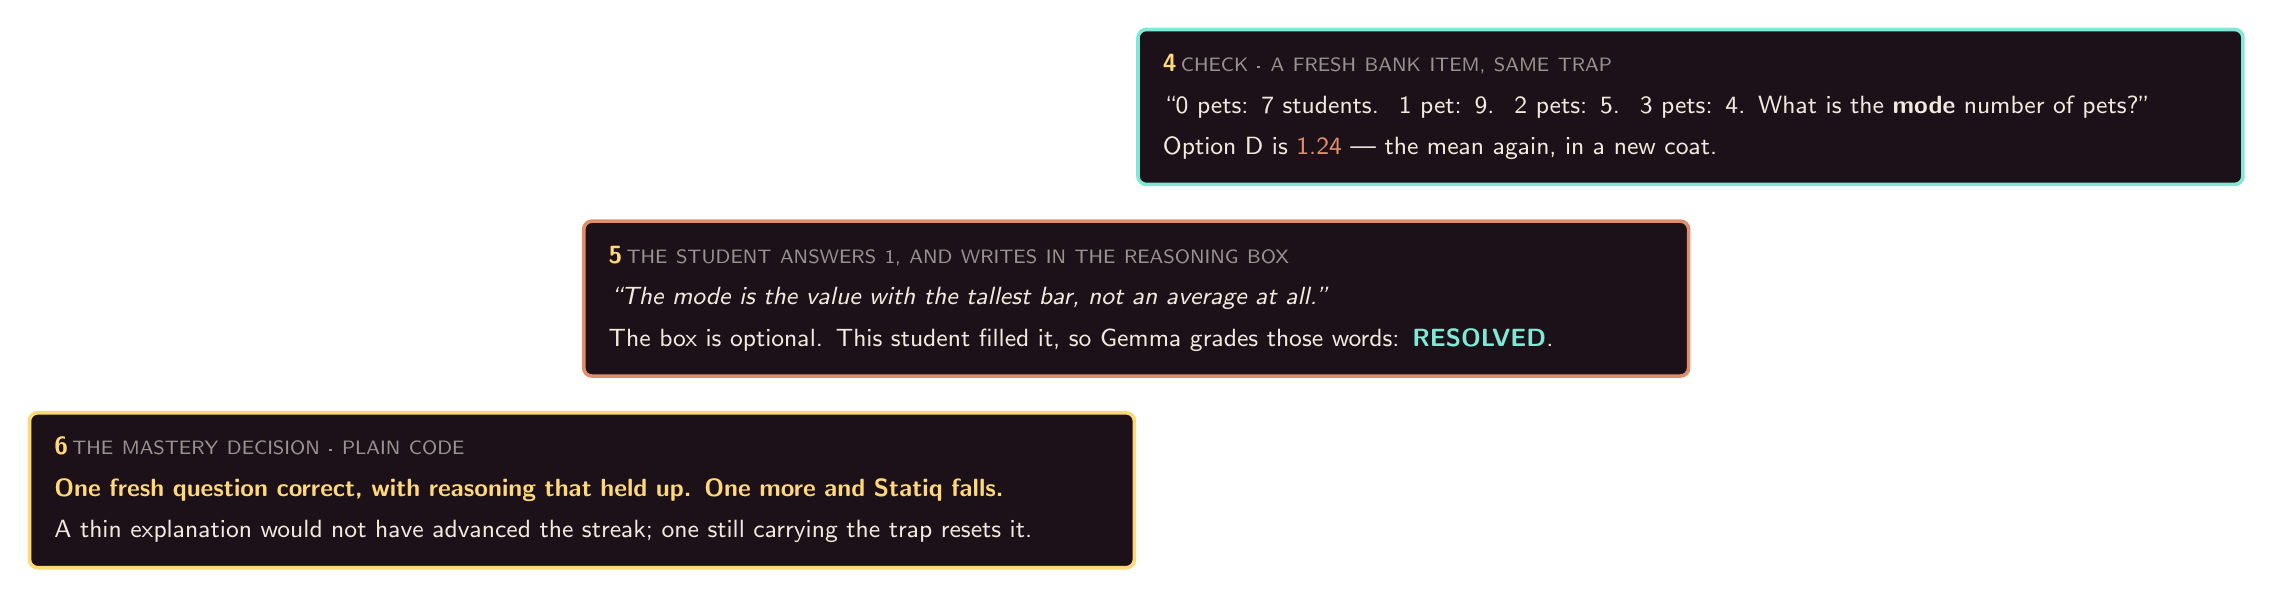
\begin{tikzpicture}[bx/.style={inner sep=9pt, align=left, font=\small,
                                 text width=13.4cm, minimum height=1.9cm},
                      every node/.append style={anchor=north west}]
    \node[codebox, bx] (c) at (0,0)
      {\stepno{4}\lbl{check · a fresh bank item, same trap}\\[4pt]
       ``0 pets: 7 students. \;1 pet: 9. \;2 pets: 5. \;3 pets: 4.
       What is the \textbf{mode} number of pets?''\\[4pt]
       Option D is \textcolor{coral}{1.24} --- the mean again, in a new coat.};
    \node[gembox, bx, below=0.42cm of c.south west] (r)
      {\stepno{5}\lbl{the student answers 1, and writes in the reasoning box}\\[4pt]
       \emph{``The mode is the value with the tallest bar, not an average at all.''}\\[4pt]
       The box is optional. This student filled it, so Gemma grades those words: \tealb{RESOLVED}.};
    \node[goldbox, bx, below=0.42cm of r.south west] (d)
      {\stepno{6}\lbl{the mastery decision · plain code}\\[4pt]
       \goldb{One fresh question correct, with reasoning that held up. One more and Statiq falls.}\\[4pt]
       A thin explanation would not have advanced the streak; one still carrying the trap resets it.};
  \end{tikzpicture}}
  \end{center}
  \vspace{0.5em}
  {\small\dimt{Correctness is decided by the bank's key. Only the words the student typed are
   ever handed to the model for judgment.}}
\end{frame}

% ================================================================ 7 · THE LOOP
\begin{frame}{The loop: teach until the trap stops working}
  \begin{columns}[T,onlytextwidth]
    \begin{column}{0.66\textwidth}
      \begin{center}
      \resizebox{\columnwidth}{!}{%
      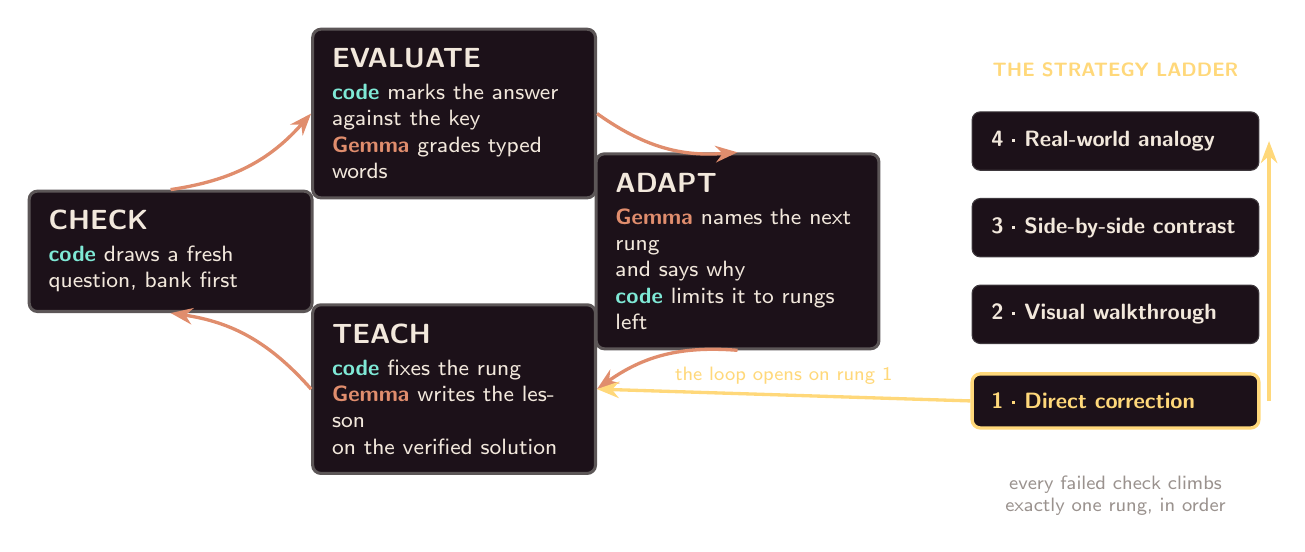
\begin{tikzpicture}[
         nd/.style={panelbox, draw=cream!35!gmbg, line width=1.1pt, align=left,
                    text width=3.1cm, minimum height=1.5cm, font=\footnotesize},
         rung/.style={panelbox, align=left, text width=3.15cm, font=\footnotesize}]
        \node[nd] (eval)  at (0,1.75)
          {\textbf{\normalsize EVALUATE}\\[2pt]
           \tealb{code} marks the answer\\ against the key\\
           \textcolor{coral}{\textbf{Gemma}} grades typed words};
        \node[nd] (adapt) at (3.6,0)
          {\textbf{\normalsize ADAPT}\\[2pt]
           \textcolor{coral}{\textbf{Gemma}} names the next rung\\ and says why\\
           \tealb{code} limits it to rungs left};
        \node[nd] (teach) at (0,-1.75)
          {\textbf{\normalsize TEACH}\\[2pt]
           \tealb{code} fixes the rung\\
           \textcolor{coral}{\textbf{Gemma}} writes the lesson\\ on the verified solution};
        \node[nd] (check) at (-3.6,0)
          {\textbf{\normalsize CHECK}\\[2pt]
           \tealb{code} draws a fresh\\ question, bank first};
        \draw[arr] (teach.west)  to[bend right=20] (check.south);
        \draw[arr] (check.north) to[bend right=20] (eval.west);
        \draw[arr] (eval.east)   to[bend right=20] (adapt.north);
        \draw[arr] (adapt.south) to[bend right=20] (teach.east);
        % the strategy ladder, read bottom-up
        \node[rung] (l4) at (8.4,1.4)  {\textbf{4 · Real-world analogy}};
        \node[rung] (l3) at (8.4,0.3)  {\textbf{3 · Side-by-side contrast}};
        \node[rung] (l2) at (8.4,-0.8) {\textbf{2 · Visual walkthrough}};
        \node[rung, draw=gold, line width=1.2pt] (l1) at (8.4,-1.9)
          {\textbf{\color{gold}1 · Direct correction}};
        \node[font=\scriptsize\bfseries, text=gold] at (8.4,2.3) {THE STRATEGY LADDER};
        \draw[garr] (l1.west) -- (teach.east)
          node[midway, above, font=\scriptsize, text=gold] {the loop opens on rung 1};
        \draw[garr] (10.35,-1.9) -- (10.35,1.4);
        \node[font=\scriptsize, text=cream!62!gmbg, align=center, text width=3.6cm]
          at (8.4,-3.1) {every failed check climbs\\ exactly one rung, in order};
      \end{tikzpicture}}
      \end{center}
    \end{column}
    \begin{column}{0.32\textwidth}
      \vspace{0.2em}
      {\scriptsize \textcolor{coral}{\textbf{Coral = Gemma judges.}} \tealb{Teal = code guarantees.}
      Most steps are both, so each node names its two halves.\par
      \vspace{0.45em}
      \textbf{Deterministic spine.} Plain code runs the loop and owns every transition;
      Gemma is called only at the judgment points.\par
      \vspace{0.4em}
      \textbf{The bar:} \goldb{two fresh questions correct in a row.} When the student
      explains their thinking, that explanation is graded, and a thin one does not
      advance the streak.\par
      \vspace{0.4em}
      \textbf{Three independent stops:} 4 check attempts, 12 model calls, a spent ladder.
      Any one ends the session, so it cannot loop forever.\par
      \vspace{0.4em}
      \dimt{Every change of strategy is announced on screen, with its reason.}\par}
    \end{column}
  \end{columns}
\end{frame}

% ================================================================ 8 · REASONING GATE
\begin{frame}{When the student explains, the explanation is graded}
  The reasoning box is optional --- leaving it blank never blocks anyone. Fill it in, and
  those words decide whether the streak moves.\par
  \vspace{0.4em}
  \begin{columns}[T,onlytextwidth]
    \begin{column}{0.5\textwidth}
      \begin{center}
      \begin{tikzpicture}
        \node[panelbox, align=left, text width=6.1cm, font=\scriptsize] {
          \lbl{the check question}\\[1pt]
          Calculate $\tfrac{1}{2}+\tfrac{1}{3}$ \;---\; picks $\tfrac{5}{6}$\, \textcolor{teal}{(correct)}\\[5pt]
          \lbl{the student types}\\[1pt]
          \emph{``I just guessed the biggest one''}\\[5pt]
          \lbl{the grade}\\[1pt]
          {\color{coral}\textbf{SHALLOW}} --- the streak does \textbf{not} advance\\[5pt]
          \lbl{the citadel answers back}\\[1pt]
          \emph{``Luck is a coin, challenger. The monsters ahead do not take coins.''}};
      \end{tikzpicture}
      \end{center}
    \end{column}
    \begin{column}{0.47\textwidth}
      {\scriptsize
      \begin{itemize}\setlength\itemsep{0.45em}
        \item Three labels, nothing else --- \textbf{RESOLVED / SHALLOW / SAME\_ERROR}.
              A closed set the model chooses from, never open-ended prose.
        \item \textbf{SAME\_ERROR} on a \emph{right} answer resets the streak: correct
              answer, but the thinking underneath it walked into the same trap.
        \item The citadel replies \goldb{to the student's own words}, in character ---
              effort met seriously, a joke met with a warning.
        \item \tealb{It fails open.} Any parse problem returns RESOLVED, so a model
              hiccup can never cost the student anything.
      \end{itemize}}
    \end{column}
  \end{columns}
\end{frame}

% ================================================================ 9 · DIRECTOR
\begin{frame}{The agent decides where the student goes next}
  \begin{center}
  \resizebox{0.99\textwidth}{!}{%
  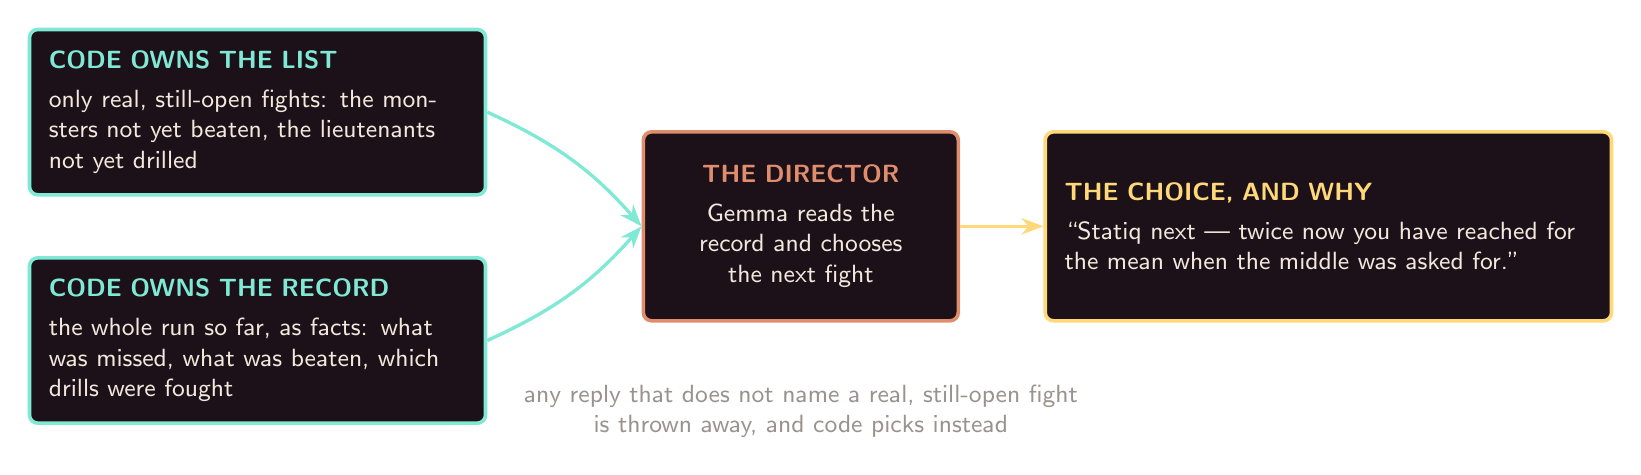
\begin{tikzpicture}
    \node[codebox, align=left, text width=5.3cm, minimum height=2.1cm] (cand) at (0,1.45)
      {\tealb{CODE OWNS THE LIST}\\[3pt]
       only real, still-open fights: the monsters not yet beaten, the lieutenants
       not yet drilled};
    \node[codebox, align=left, text width=5.3cm, minimum height=2.1cm] (evid) at (0,-1.45)
      {\tealb{CODE OWNS THE RECORD}\\[3pt]
       the whole run so far, as facts: what was missed, what was beaten, which
       drills were fought};
    \node[gembox, minimum width=4.0cm, minimum height=2.4cm, text width=3.5cm] (dir) at (6.9,0)
      {\textbf{\textcolor{coral}{THE DIRECTOR}}\\[3pt]
       Gemma reads the record and chooses the next fight};
    \node[goldbox, align=left, text width=6.7cm, minimum height=2.4cm] (out) at (13.6,0)
      {\goldb{THE CHOICE, AND WHY}\\[3pt]
       ``Statiq next --- twice now you have reached for the mean when the middle
       was asked for.''};
    \draw[tarr] (cand.east) to[bend left=12] (dir.west);
    \draw[tarr] (evid.east) to[bend right=12] (dir.west);
    \draw[garr] (dir.east) -- (out.west);
    \node[font=\small, text=cream!62!gmbg, align=center, text width=7.6cm] at (6.9,-2.35)
      {any reply that does not name a real, still-open fight\\ is thrown away, and code picks instead};
  \end{tikzpicture}}
  \end{center}
  \vspace{0.45em}
  {\large Everywhere else Gemma answers one question. Here it \goldb{shapes the session} ---
   and it must name the evidence it used.\par}
  \vspace{0.3em}
  \dimt{\small The record it sees is complete, so it cannot invent a history the student never had.}
\end{frame}

% ================================================================ 10 · ARCHITECTURE
\begin{frame}{Everything on one laptop}
  \begin{center}
  \resizebox{0.82\textwidth}{!}{%
  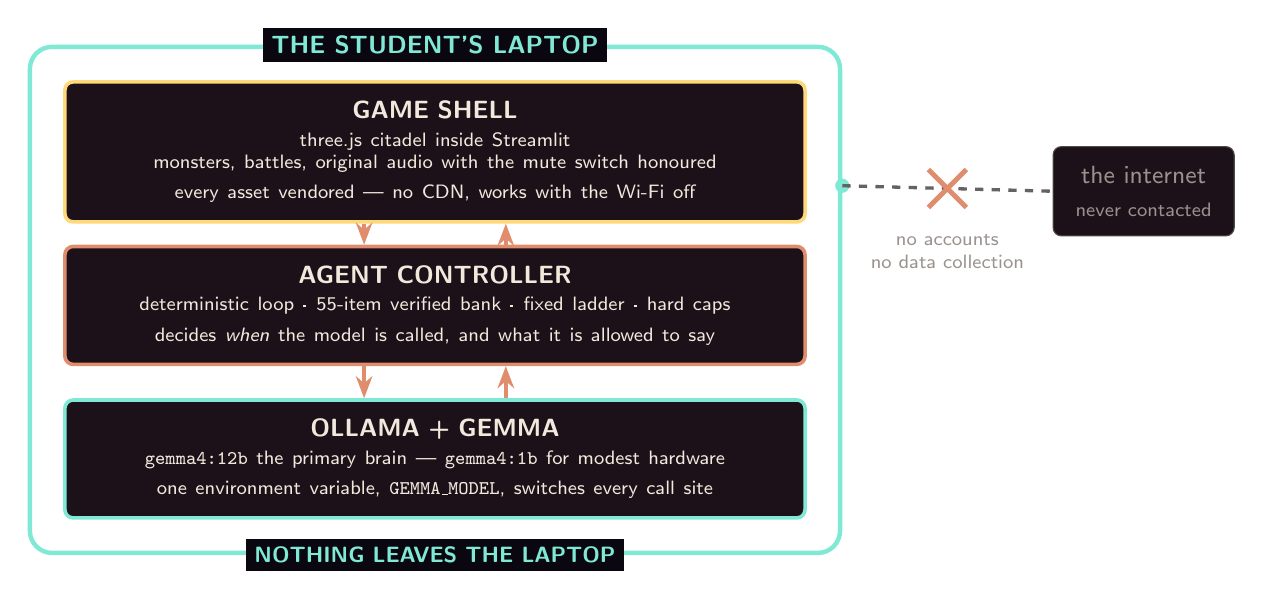
\begin{tikzpicture}
    \node[goldbox, minimum width=9.4cm, text width=8.8cm] (game) at (0,2.5)
      {\textbf{GAME SHELL}\\[2pt]\scriptsize three.js citadel inside Streamlit\\
       \scriptsize monsters, battles, original audio with the mute switch honoured\\
       \scriptsize every asset vendored --- no CDN, works with the Wi-Fi off};
    \node[gembox, minimum width=9.4cm, text width=8.8cm] (agent) at (0,0.55)
      {\textbf{AGENT CONTROLLER}\\[2pt]\scriptsize deterministic loop · 55-item verified bank · fixed ladder · hard caps\\
       \scriptsize decides \emph{when} the model is called, and what it is allowed to say};
    \node[codebox, minimum width=9.4cm, text width=8.8cm] (gemma) at (0,-1.4)
      {\textbf{OLLAMA + GEMMA}\\[2pt]\scriptsize \texttt{gemma4:12b} the primary brain --- \texttt{gemma4:1b} for modest hardware\\
       \scriptsize one environment variable, \texttt{GEMMA\_MODEL}, switches every call site};
    \draw[arr] ($(game.south)+(-0.9,0)$) -- ($(agent.north)+(-0.9,0)$);
    \draw[arr] ($(agent.north)+(0.9,0)$) -- ($(game.south)+(0.9,0)$);
    \draw[arr] ($(agent.south)+(-0.9,0)$) -- ($(gemma.north)+(-0.9,0)$);
    \draw[arr] ($(gemma.north)+(0.9,0)$) -- ($(agent.south)+(0.9,0)$);
    % the boundary
    \node[draw=teal, line width=1.6pt, rounded corners=8pt, inner sep=12pt,
          fit=(game)(gemma)] (laptop) {};
    \node[font=\small\bfseries, text=teal, fill=gmbg, inner sep=3pt]
      at (laptop.north) {THE STUDENT'S LAPTOP};
    \node[font=\footnotesize\bfseries, text=teal, fill=gmbg, inner sep=3pt]
      at (laptop.south) {NOTHING LEAVES THE LAPTOP};
    % the internet, unreachable -- the dashed line leaves the laptop boundary itself
    \coordinate (edge) at ($(laptop.east)+(0,1.45)$);
    \node[panelbox, draw=cream!30!gmbg, minimum width=2.3cm, text=cream!62!gmbg]
      (net) at (9.0,2.0) {the internet\\[1pt]\scriptsize never contacted};
    \fill[teal] (edge) circle (0.09);
    \draw[line width=1.2pt, color=cream!40!gmbg, dashed] (edge) -- (net.west);
    \node[cross out, draw=coral, line width=1.8pt, minimum size=0.42cm]
      at ($(edge)!0.5!(net.west)$) {};
    \node[font=\scriptsize, text=cream!62!gmbg, align=center]
      at ($(edge)!0.5!(net.west)+(0,-0.8)$) {no accounts\\ no data collection};
  \end{tikzpicture}}
  \end{center}
  \vspace{0.35em}
  \begin{center}
  {\small Every asset is vendored into \texttt{static/}. The only network call the code
   makes is to \goldb{Ollama on localhost}, and the letters home are written to a file
   on the same machine.}
  \end{center}
\end{frame}

% ================================================================ 11 · TRUST SPLIT
\begin{frame}{Gemma judges. Code guarantees.}
  \begin{center}
  \resizebox{0.92\textwidth}{!}{%
  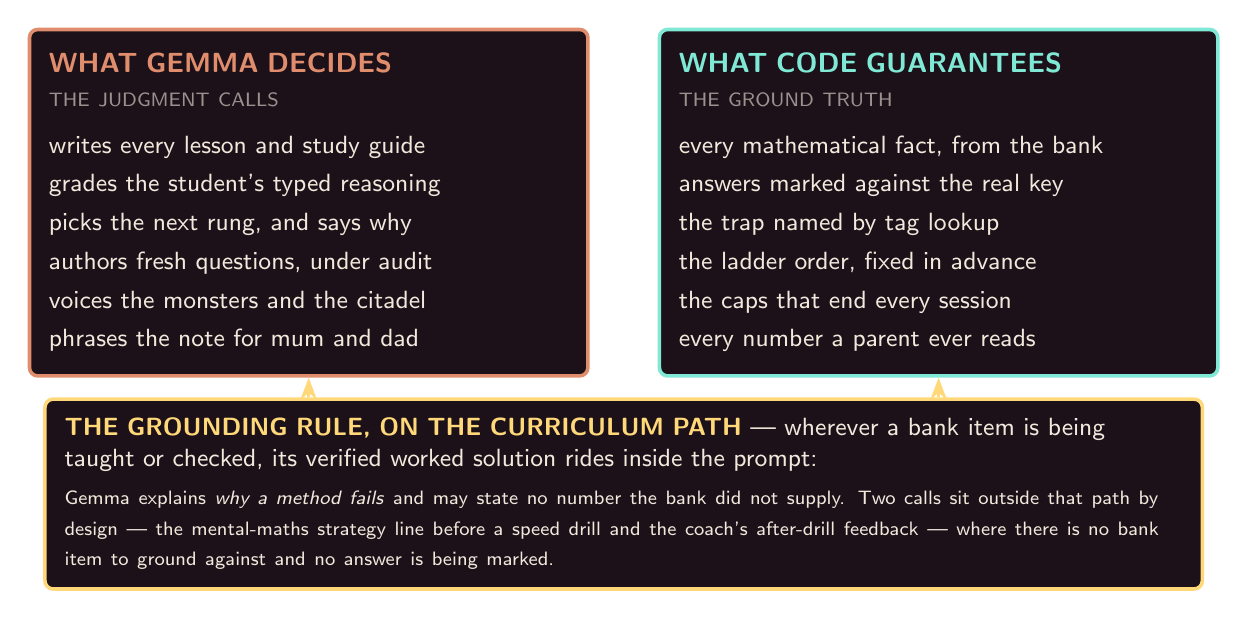
\begin{tikzpicture}
    \node[gembox, align=left, text width=6.6cm, minimum height=4.4cm, font=\small] (gem) at (0,0) {
      {\normalsize\textbf{\textcolor{coral}{WHAT GEMMA DECIDES}}}\\[1pt]
      \lbl{the judgment calls}\\[6pt]
      writes every lesson and study guide\\[3pt]
      grades the student's typed reasoning\\[3pt]
      picks the next rung, and says why\\[3pt]
      authors fresh questions, under audit\\[3pt]
      voices the monsters and the citadel\\[3pt]
      phrases the note for mum and dad};
    \node[codebox, align=left, text width=6.6cm, minimum height=4.4cm, font=\small] (cod) at (8.0,0) {
      {\normalsize\textbf{\textcolor{teal}{WHAT CODE GUARANTEES}}}\\[1pt]
      \lbl{the ground truth}\\[6pt]
      every mathematical fact, from the bank\\[3pt]
      answers marked against the real key\\[3pt]
      the trap named by tag lookup\\[3pt]
      the ladder order, fixed in advance\\[3pt]
      the caps that end every session\\[3pt]
      every number a parent ever reads};
    \node[goldbox, align=left, minimum width=14.7cm, text width=14.2cm, font=\small]
      (bank) at (4.0,-3.7)
      {\goldb{THE GROUNDING RULE, ON THE CURRICULUM PATH} --- wherever a bank item is being
       taught or checked, its verified worked solution rides inside the prompt:\\[3pt]
       \scriptsize Gemma explains \emph{why a method fails} and may state no number the bank
       did not supply. Two calls sit outside that path by design --- the mental-maths
       strategy line before a speed drill and the coach's after-drill feedback --- where
       there is no bank item to ground against and no answer is being marked.};
    \draw[garr] (bank.north -| gem) -- (gem.south);
    \draw[garr] (bank.north -| cod) -- (cod.south);
  \end{tikzpicture}}
  \end{center}
  \vspace{0.2em}
  {\small Every mathematical fact a student is graded on comes from the bank ---
   \goldb{never from the model}.}
\end{frame}

% ================================================================ 12 · DESIGNED TO FAIL
\begin{frame}{Designed for the model to fail}
  Four things the model actually did in testing --- and the structure that now stands in the way.\par
  \vspace{0.45em}
  \begin{center}
  \resizebox{0.965\textwidth}{!}{%
  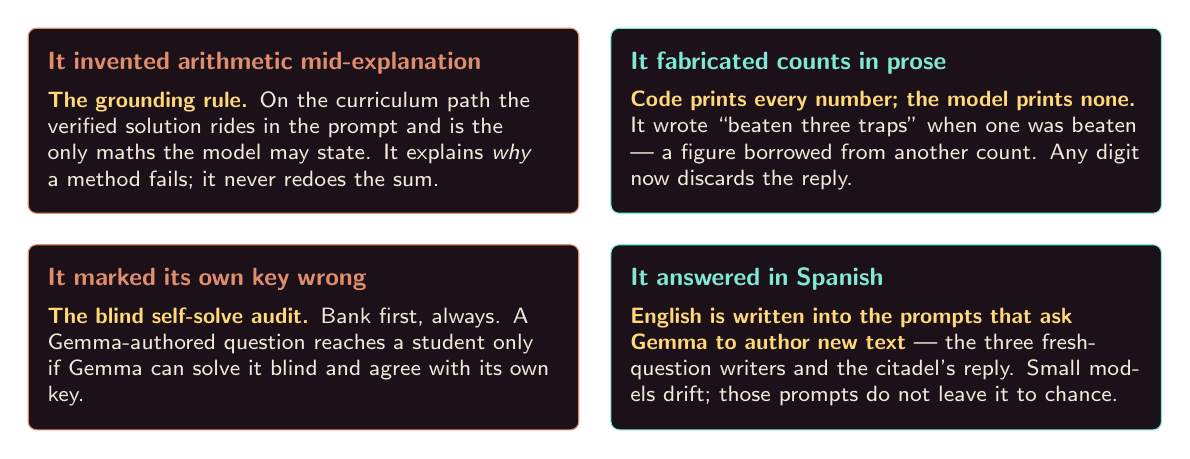
\begin{tikzpicture}[card/.style={panelbox, align=left, text width=6.5cm,
                                   minimum height=2.35cm, inner sep=7pt, font=\footnotesize}]
    \node[card, draw=coral] (a) at (0,0)
      {{\small\textbf{\textcolor{coral}{It invented arithmetic mid-explanation}}}\\[4pt]
       \goldb{The grounding rule.} On the curriculum path the verified solution rides in
       the prompt and is the only maths the model may state. It explains \emph{why} a
       method fails; it never redoes the sum.};
    \node[card, draw=teal] (b) at (7.4,0)
      {{\small\textbf{\textcolor{teal}{It fabricated counts in prose}}}\\[4pt]
       \goldb{Code prints every number; the model prints none.} It wrote ``beaten three
       traps'' when one was beaten --- a figure borrowed from another count. Any digit
       now discards the reply.};
    \node[card, draw=coral] (c) at (0,-2.75)
      {{\small\textbf{\textcolor{coral}{It marked its own key wrong}}}\\[4pt]
       \goldb{The blind self-solve audit.} Bank first, always. A Gemma-authored question
       reaches a student only if Gemma can solve it blind and agree with its own key.};
    \node[card, draw=teal] (d) at (7.4,-2.75)
      {{\small\textbf{\textcolor{teal}{It answered in Spanish}}}\\[4pt]
       \goldb{English is written into the prompts that ask Gemma to author new text} ---
       the three fresh-question writers and the citadel's reply. Small models drift; those
       prompts do not leave it to chance.};
  \end{tikzpicture}}
  \end{center}
  \vspace{0.4em}
  {\small\color{gold} The structure carries correctness. Model size still shows: the 1B
   under-detects thin reasoning that the 12B catches, on the same prompts.}
\end{frame}

% ================================================================ 13 · PARENTS
\begin{frame}{The part that reaches the kitchen table}
  \begin{columns}[T,onlytextwidth]
    \begin{column}{0.49\textwidth}
      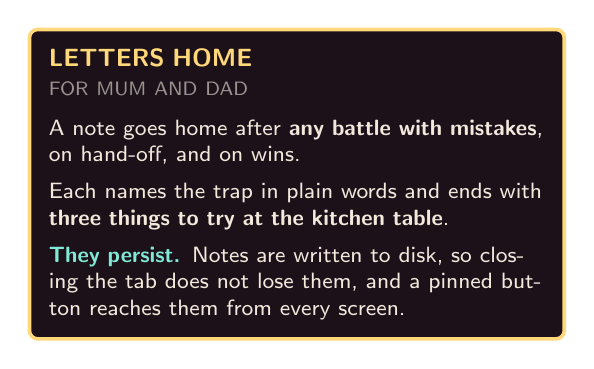
\begin{tikzpicture}
        \node[goldbox, align=left, text width=6.3cm, minimum height=3.5cm, font=\footnotesize] {
          {\small\textbf{\textcolor{gold}{LETTERS HOME}}}\\[1pt]
          \lbl{for mum and dad}\\[5pt]
          A note goes home after \textbf{any battle with mistakes}, on hand-off,
          and on wins.\\[4pt]
          Each names the trap in plain words and ends with \textbf{three things to
          try at the kitchen table}.\\[4pt]
          \tealb{They persist.} Notes are written to disk, so closing the tab does
          not lose them, and a pinned button reaches them from every screen.};
      \end{tikzpicture}
    \end{column}
    \begin{column}{0.49\textwidth}
      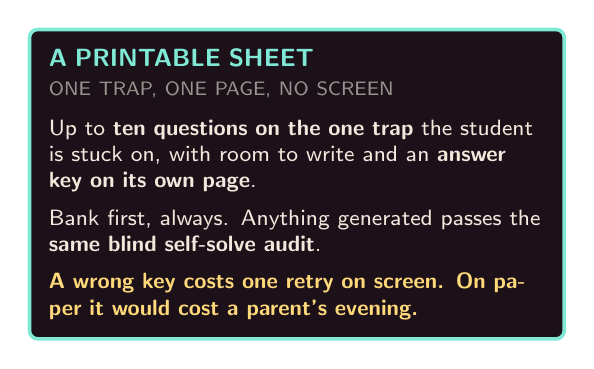
\begin{tikzpicture}
        \node[codebox, align=left, text width=6.3cm, minimum height=3.5cm, font=\footnotesize] {
          {\small\textbf{\textcolor{teal}{A PRINTABLE SHEET}}}\\[1pt]
          \lbl{one trap, one page, no screen}\\[5pt]
          Up to \textbf{ten questions on the one trap} the student is stuck on, with
          room to write and an \textbf{answer key on its own page}.\\[4pt]
          Bank first, always. Anything generated passes the \textbf{same blind
          self-solve audit}.\\[4pt]
          \goldb{A wrong key costs one retry on screen. On paper it would cost a
          parent's evening.}};
      \end{tikzpicture}
    \end{column}
  \end{columns}
  \vspace{0.4em}
  \begin{center}
  {\small Every number a parent reads is \goldb{computed in code}. Gemma only says what they mean.\par}
  \end{center}
\end{frame}

% ================================================================ 14 · THE GAME
\begin{frame}{And a fourteen-year-old wants to play it}
  \begin{center}
  \resizebox{0.985\textwidth}{!}{%
  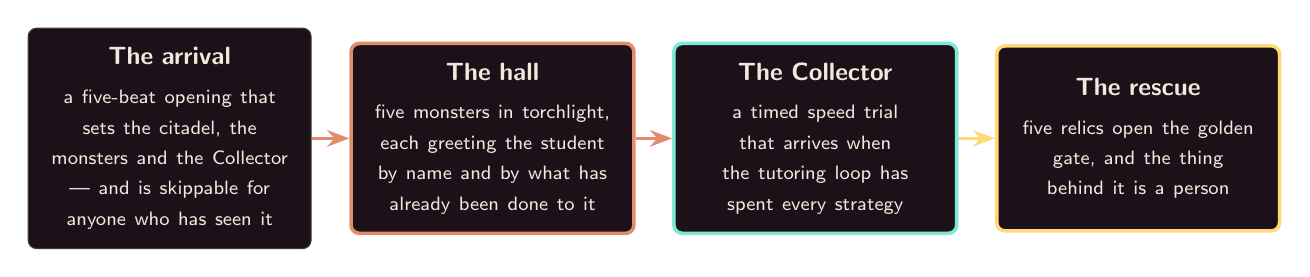
\begin{tikzpicture}[bx/.style={minimum height=2.35cm, text width=3.1cm, font=\small}]
    \node[panelbox, bx] (a) at (0,0)
      {\textbf{The arrival}\\[3pt]\scriptsize a five-beat opening
       that sets the citadel, the monsters and the Collector --- and is
       skippable for anyone who has seen it};
    \node[gembox, bx] (b) at (4.1,0)
      {\textbf{The hall}\\[3pt]\scriptsize five monsters in torchlight,
       each greeting the student by name and by what has already been done to it};
    \node[codebox, bx] (c) at (8.2,0)
      {\textbf{The Collector}\\[3pt]\scriptsize a timed speed trial
       that arrives when the tutoring loop has spent every strategy};
    \node[goldbox, bx] (d) at (12.3,0)
      {\textbf{The rescue}\\[3pt]\scriptsize five relics open the golden
       gate, and the thing behind it is a person};
    \draw[arr] (a) -- (b);
    \draw[arr] (b) -- (c);
    \draw[garr] (c) -- (d);
  \end{tikzpicture}}
  \end{center}
  \vspace{0.7em}
  \begin{itemize}\setlength\itemsep{0.42em}
    \item The Collector keeps \textbf{three lieutenants} --- Twinfang for doubling and
          halving, The Niner for nines, Splitjaw for making tens. Ninety seconds each,
          and a Gemma coach that reads \goldb{the actual misses} rather than the score.
    \item Original audio throughout, and the \textbf{mute switch is honoured everywhere},
          including the places nobody checks.
  \end{itemize}
\end{frame}

% ================================================================ 15 · CLOSE
\begin{frame}
  \begin{center}
    \vspace{1.5em}
    {\fontsize{26}{32}\selectfont\bfseries\color{cream} Find the idea behind the wrong answer.\\
     Teach until the student can show it is gone.\par}
    \vspace{0.9em}
    {\Large\color{gold} Bank-grounded, hard-capped, and entirely on one laptop.\par}
    \vspace{1.1em}
    \dimt{\large A student who adds fractions straight across meets Fractis, is taught on a
    fixed ladder of four strategies, and the loop ends one of two ways --- two fresh questions
    correct in a row, or a note written home. Nothing about them ever leaves their laptop.}\par
    \vspace{1.3em}
    {\small\color{teal} github.com/EdTechDL/gemma-without-borders \,·\, live demo, Wi-Fi off \,·\, Kaggle notebook}\par
    \vspace{0.5em}
    {\small Gokulakrishnan \,\textcolor{coral}{·}\, Padmanabha \,\textcolor{coral}{·}\, Taha \,\textcolor{coral}{·}\, Naimah \,\textcolor{coral}{·}\, Amarah}
  \end{center}
\end{frame}

\end{document}
